	\chapter{Monte--Carlo--Integration}\label{chapter:mc_integration}
	Monte--Carlo--Verfahren liegt die Idee zugrunde, zu einem numerischen Problem ein passendes Zufallsexperiment so zu konstruieren, so dass der Erwartungswert einer Zufallsvariable des Experiments das numerische Problem löst.
	
	Die Idee ist nicht neu, so fÜhrte {\em Buffon} 1777 folgendes Experiment durch: Eine Nadel der LÄnge $L$ wird wiederholt auf eine plane FlÄche mit parallelen Linien im Abstand $d>L$ fallengelassen und jeweils notiert, ob die Nadel eine der Linien kreuzt. Er zeigte, dass der Erwartungswert fÜr die Wahrscheinlichkeit der Nadel, die Linie zu kreuzen $$p=\frac{2L}{\pi d}$$ betrÄgt. Laplace wies spÄter darauf hin, dass  man die HÄufigkeit, mit der die Nadeln die Linien kreuzen, auch Nutzen kann, um den Wert von $\pi$ zu schÄtzen (siehe Abb. \ref{fig:buffon}): $$\pi=\frac{2L}{p d}\approx \frac{2L}{\frac{k}{N}d}$$
	(\text{N Experimente, davon k mal eine Linie gekreuzt}).
	\begin{figure}
		\centering
		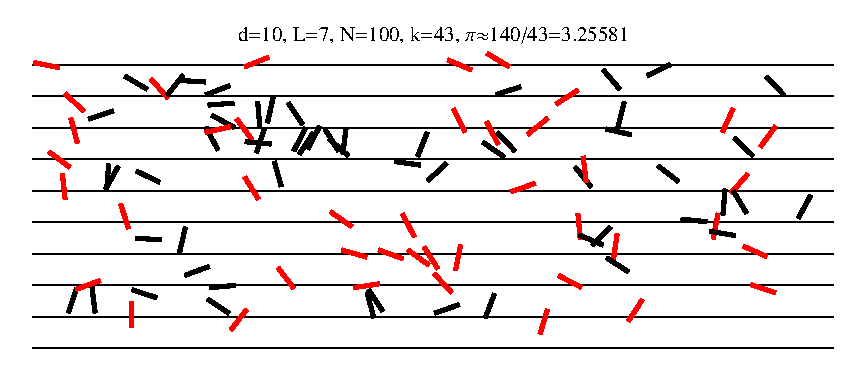
\includegraphics[height=0.3\textheight]{buffonsneedles.eps}
		\caption{Beispiel fÜr eine Realisierung des Buffon--Nadel--Experiments mit 100 geworfenen Nadeln. Der erhaltene SchÄtzwert fÜr $\pi$ ist bei so wenigen Nadeln nicht sehr genau.}
		\label{fig:buffon}
	\end{figure}
	
	\section{Das Integrationsproblem}\label{subsec:integrationsproblem}
	Betrachten wir das Integral
	\begin{equation}
		I=\int_\Omega f(x) d\mu(x),
		\label{eq:integration_problem}
	\end{equation}
	wobei $\Omega$ das Integrationsgebiet, $f : \Omega \to \mathbb{R}$ eine reellwertige Funktion und $\mu$ ein Ma"s auf $\Omega$ ist. FÜr die folgende Darstellung nehmen wir an, dass $$\Omega=[0,1]^d$$ der $d$--dimensionale EinheitswÜrfel und $I_d$ das zugehörige Integral ist.
	\subsection{Klassische numerische Quadraturverfahren}
	Die klassische numerische Herangehensweise (wenn keine analytische Lösung möglich oder praktikabel ist) sind {\em Tensor--Produkt--Verfahren}. Die Idee dabei ist, fÜr jede Dimension ein eindimensionales Quadratur--Verfahren zu wÄhlen (verschiedene oder das gleiche) und diese zu einem mehrdimensionalen Verfahren zu kombinieren. Ein eindimensionales Verfahren stellt eine gewichtete Summe von Funktionswerten an $M$ (vor dem Auswerten der Funktion) festgelegten StÜtzstellen dar:
	$${\tilde I}_1=\sum_{i=1}^M w_i\,f(x_i).$$
	Bekannte Vertreter dieser eindimensionalen Quadraturregeln sind z.B. die {\em Newton--Cotes}- und {\em Gauss--Legendre}--Verfahren. Ein hieraus konstruiertes Tensor--Produkt--Verfahren (wobei wir der Einfachheit halber fÜr alle Dimensionen dasselbe eindimensionale Verfahren zugrundelegen) hat dann die Form:
	$${\tilde I}_d^{\,\text{TP}}=\sum_{i_1}^M\cdots\sum_{i_d}^M w_{i_1}w_{i_2}\cdots w_{i_d}f(x_{i_1},\cdots,x_{i_d}).$$
	Aus einem eindimensionalen Verfahren mit $M$ StÜtzstellen erhalten wir also ein $d$--dimensionales Verfahren mit $M^d$ StÜtzstellen (Siehe Abb. {\ref{fig:tensorproduct}}).
	\begin{figure}
		\centering
		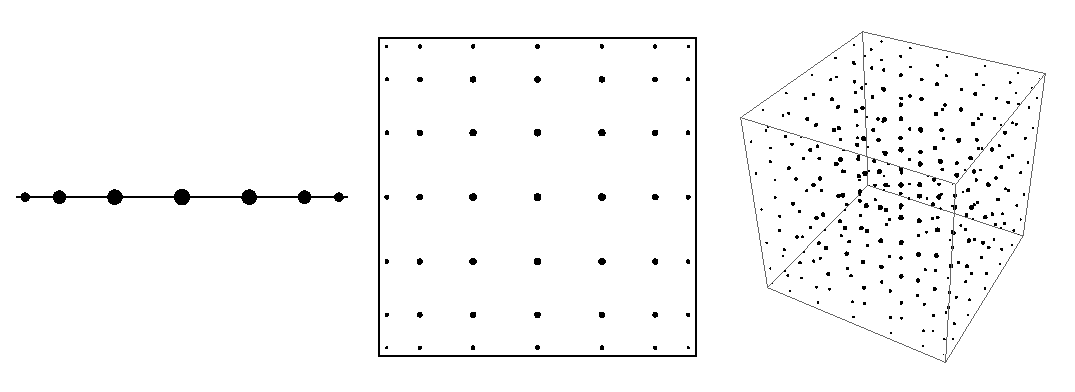
\includegraphics[height=0.25\textheight]{tensorproduct_quadrature.eps}
		\caption{StÜtzstellen eines 1D 7--Punkt--Gauss--Legendre--Verfahrens und entsprechender Tensor--Produkt--Verfahren fÜr 2 bzw. 3 Dimensionen. Die Gewichte der StÜtzstellen sind durch ihre Grö"se kenntlich gemacht.}
		\label{fig:tensorproduct}
	\end{figure}
	
	\subsection{einfache Monte--Carlo--Integration}
	Bei der Monte--Carlo--Integration ziehen wir $N$ zufÄllige, gemÄ"s einer Wahrscheinlichkeitsdichte $p$ verteilte StÜtzstellen $[X_i|i\in\{1,\dots,N\}]$ in $\Omega$ und schÄtzen dann den Wert des Integrals (\ref{eq:integration_problem}) mit
	\begin{equation}
		{\tilde I}_d^{\,\text{MC}}=\frac{1}{N}\sum_{i=0}^{N-1} \frac{f(X_i)}{p(X_i)}
		\label{eq:mc_integral}
	\end{equation}
	ab. Im Falle unseres $d$--dimensionalen EinheitswÜrfels $\Omega=[0,1]^d$ können wir besipielsweise jede StÜtzstelle aus $d$ gleichförmig auf dem Einheitsintervall $[0,1]$ verteilten Zufallszahlen $U_i$ durch einfache Tupelbildung
	$$X_i:=(U_{d i},\dots,U_{d(i+1)-1})$$
	gewinnen. Aber auch fÜr allgemeine Integrationsgebiete $\Omega$ kann das Verfahren genauso angewandt werden, solange ein passendes Integrationsma"s $\mu$ und ein Wahrscheinlichkeitsma"s $P$ existieren, so dass $$P(D)=\text{Pr}(x\in D)$$ fÜr jede me"sbare Menge $D\subset\Omega$ gilt. Die entsprechende Wahrscheinlichkeitsdichte $p$ lÄsst sich mit Hilfe der {\em Radon--Nikodym--Ableitung} $$p(x)=\frac{dP}{d\mu}(x)$$
	einfÜhren, wobei $p$ dann einfach eine Funktion ist, fÜr die $$P(D)=\int_D p(x)d\mu(x)$$ gilt.
	Von der Erwartungstreue des SchÄtzers (\ref{eq:mc_integral}) fÜr unser Integral (\ref{eq:integration_problem}) können wir uns mit \citep[][2.4]{Veach:1997p9136}
	\begin{align*}
		E[{\tilde I}_d^{\,\text{MC}}] &=E\left[\frac{1}{N}\sum_{i=0}^{N-1}\frac{f(X_i)}{p(X_i)}\right] \\
			&= \frac{1}{N}\sum_{i=0}^{N-1}E\left[\frac{f(X_i)}{p(X_i)}\right] \\
			&= \frac{1}{N}\sum_{i=0}^{N-1}\int_\Omega \frac{f(X_i)}{p(X_i)}p(X_i)\,d\mu(x) \\
			&= \int_\Omega f(x)\,d\mu(x)\\
			&= I
	\end{align*}
	leicht Überzeugen.
	
	\subsection{Konvergenzraten}\label{subsec:integrationsproblem_comparison}
	Wir wollen nun die Konvergenzraten der Tensor--Produkt--Verfahren mit der Konvergenzrate des einfachen Monte--Carlo--SchÄtzers (\ref{eq:mc_integral}) vergleichen. Zur Konstruktion eines Vertreters der Tensor--Produkt--Verfahren verwenden wir beispielhaft das Newton--Cotes--Verfahren. In \citep[][3.1.4]{Stoer:2005p10586} wird als Ab\-schÄt\-zung fÜr den Fehler eines Verfahrens $p$--ter Ordnung (d.h. ein Verfahren, das alle Polynome bis zum Grad $p$ exakt integriert) und Schrittweite $h(\approx\frac{b-a}{N}=\mathcal{O}(N^{-1}))$ der StÜtzstellen
	\begin{equation}
		\int_a^b P_n(x)-f(x)dx=h^{p+1}K f^{(p)}(\xi),\quad\xi\in(a,b)
		\label{eq:quadrature_error}
	\end{equation}
	angegeben, wobei $n$ die Anzahl der StÜtzstellen, $P_n$ das Interpolationspolynom fÜr die StÜtzstellen und K eine Konstante ist. Gauss--Legendre--Verfahren sind von der Ordnung $2n-1$, d.h. die Konvergenzrate dieser $n$--Punkt--Formel ist demnach von der Grö"senordnung $\mathcal{O}(h^{2n})=\mathcal{O}(N^{-2n})$.\footnote{$N$ bezeichnet die Anzahl der StÜtzstellen fÜr das gesamte Integrationsintervall. Der SchÄtzwert fÜr das Integral wird dann durch $\frac{N}{n}$--maliges Anwenden der $n$--Punkt--Formel berechnet}
	Durch Bildung der entsprechenden $d$--dimensionalen Tensor--Produkt--Regel Ändert sich die Konvergenzrate in Bezug auf die Schrittweite $h$ nicht. Da unsere $N$ StÜtzstellen sich nun aber auf ein $d$--dimensionales Gitter verteilen, teilt sich das Volumen unseres $d$--dimensionalen EinheitswÜrfels in $N$ WÜrfel mit einem Volumen von jeweils $h^d$ auf, d.h. fÜr die Schrittweite folgt
	$$\mathcal{O}(1)=V=N h^d \Rightarrow h=\mathcal{O}\left(\left(\frac{1}{N}\right)^{1/d}\right)=\mathcal{O}\left(N^{-1/d}\right)$$	
	und damit fÜr die Konvergenzrate in Bezug auf die GesamtstÜtzstellenzahl
	$$\mathcal{O}(h^{2n})=\mathcal{O}(N^{-2n/d}).$$
	Dies bedeutet, dass Tensor--Produktverfahren mit steigender Dimension des Integrationsgebietes an Effizienz verlieren. Bei hochdimensionalen Problemen kann dies kaum durch Verfahren höherer Ordnung ausgeglichen werden, da Verfahren höherer Ordnung, wie oben in (\ref{eq:quadrature_error}) zu sehen, auch grö"sere Anforderungen an die Glattheit der Funktion stellen. Au"serdem kann die exponentiell steigende Anzahl $N \geq n^d$ mindestens nötiger Funktionsaufrufe zu einem Problem werden. Der Effekt wird bei steigender Dimension und Ordnung des Verfahrens nur noch schlimmer, was ein Ausgleichen der schlechteren Konvergenzrate bei höheren Dimensionen durch Erhöhen der Ordnung des Verfahrens schnell praktisch unmöglich werden lÄsst. Dies wird hÄufig als {\em Curse~of~Dimensionality} (Fluch der DimensionalitÄt) bezeichnet.
	
	Bei der Monte--Carlo--Integration können wir die Konvergenzrate anhand der Varianz unseres Monte--Carlo--SchÄtzers (\ref{eq:mc_integral}) bestimmen \citep[][2.4.1]{Veach:1997p9136}. Nennen wir der Übersicht wegen
	$$Y_i=\frac{f(X_i)}{p(X_i)}$$
	und den MC--SchÄtzer mit $N$ gezogenenen Werten
	$$F_N=\frac{1}{N}\sum_{i=0}^{N-1} Y_i.$$
	Dann gilt fÜr die Varianz eines beliebigen Samples
	\begin{equation}
		V[Y_i]=E[(Y_i-E[Y_i])^2]=E[Y_i^2]-E[Y_i]^2=\int_\Omega \frac{f(x)^2}{p(x)}d\mu(x)-I^2.
		\label{eq:mc_variance}
	\end{equation}
	Da die Werte unabhÄngig gezogen sind, gilt fÜr die Varianz des SchÄtzer mit $N$ Werten
	$$V[F_N]=V\left[\frac{1}{N}\sum_{i=0}^{N-1}Y_i\right]=\frac{1}{N^2}V\left[\sum_{i=0}^{N-1}Y_i\right]=\frac{1}{N^2}\sum_{i=0}^{N-1}V[Y_i]=\frac{1}{N}V[Y_i],$$
	d.h. die Varianz des SchÄtzers sinkt invers mit der Anzahl $N$ an gezogenen Werten. Daraus folgt sofort die Standardabweichung
	\begin{equation}
		\sigma[F_N]=\frac{1}{\sqrt{N}}\sigma[Y_i],
		\label{eq:mc_standarddeviation}
	\end{equation}
	was einer Konvergenzrate von $\mathcal{O}(N^{-1/2})$ entspricht. Die Konvergenzrate des Monte--Carlo--SchÄtzers ist im Gegensatz zur Konvergenzrate der Tensor--Produkt--Verfahren also unabhÄngig von der Dimension des Integrationsgebietes, d.h. das Verfahren leidet {\em nicht} unter dem {\em Curse~of~Dimensionality}! Au"serdem mussten wir nirgendwo Bedingungen an die Glattheit der Funktion stellen, was bei Funktionen mit DiskontinuitÄten von Vorteil ist.
	
	Zusammenfassend können wir also feststellen, dass Monte--Carlo--Integration bei hochdimensionalen Integrationsproblemen und Funktionen mit DiskontinuitÄten klar gegenÜber klassischen Tensor--Produktverfahren vorzuziehen ist. FÜr niedrigdimensionale ($d\lessapprox 7$) Gebiete mit glatten Integranden sind die klassischen Methoden hingegen besser geeignet.
	
	
	\section{Importance--Sampling}\label{subsec:importancesampling}
	Wir sind bei unserem MC--SchÄtzer (\ref{eq:mc_integral}) nicht darauf beschrÄnkt eine gleich\-för\-mi\-ge Wahrscheinlichkeitsdichte $p$ zu wÄhlen. Es kann die Effizienz des Verfahrens sogar betrÄchtlich verbessern, wenn wir eine geeignete Wahrscheinlichkeitsdichte $p$ wÄhlen. Schauen wir uns daher die Formel (\ref{eq:mc_variance}) fÜr die Varianz, die es zu minimieren gilt, nochmal an, um zu verstehen, was ``geeignet'' bedeutet. Nimmt die Wahrscheinlichkeitsdichte beispielsweise die ideale Form
	\begin{equation}
		p(x)=\frac{|f(x)|}{\int_\Omega |f(z)|d\mu(z)}
		\label{eq:ideal_importance_pdf}
	\end{equation}
	an, kann man mit der {\em Jensenschen~Ungleichung} zeigen, dass dann das Integral in (\ref{eq:mc_variance}) und damit die Varianz insgesamt minimal wird. Nimmt $f$ keine negativen Werte an, verschwindet die Varianz dieses SchÄtzers sogar, da in (\ref{eq:mc_integral}) dann nur noch Über die konstante Lösung (in Form der Normierungskonstanten) gemittelt wird. Wenn wir das Normierungs--Integral im Nenner von (\ref{eq:ideal_importance_pdf}) lösen könnten, wÄre allerdings auch die ursprÜngliche Integration (\ref{eq:integration_problem}) kein Problem! Daher suchen wir in der Praxis nach einem $p$, das möglichst Ähnlich zu $|f|$ und gleichzeitig normierbar ist.
	
